% ---------------------------------------------------------------------------------------------------------------
% TEMPLATE PARA PROPOSTA DE TRABALHO DE CONCLUSÃO DE CURSO
% Universidade Tecnológica Federal do Paraná - UTFPR
% Customização da classe abnTeX2 (http://www.abntex.net.br/) para as normas da UTFPR
%
% Projeto: http://tcc.tsi.gp.utfpr.edu.br/paginas/modelos-latex-da-utfpr
% Autores: Diego Marczal
% 	   Michael Vornes <https://github.com/mvornes>
%
%----------------------------------------------------------------------------------------------------------------
% Codificação: UTF-8
% LaTeX:  abnTeX2          
% ---------------------------------------------------------------------------------------------------------------


% CARREGA CLASSE PERSONALIZADA DA UTFPR--------------------------------------------------------------------------
\documentclass[%twoside,                   % Impressão em frente e verso
    	        oneside,                   % Impressão apenas frente
]{configuracoes/utfpr-abntex2}


% INCLUI ARQUIVOS DE CONFIGURAÇÕES-------------------------------------------------------------------------------
% REFERÊNCIAS-----------------------------------------------------------------
\usepackage[%
    alf,
    abnt-emphasize=bf,
    bibjustif,
    recuo=0cm,
    abnt-url-package=url,       % Utiliza o pacote url
    abnt-refinfo=yes,           % Utiliza o estilo bibliográfico abnt-refinfo
    abnt-etal-cite=3,
    abnt-etal-list=3,
    abnt-thesis-year=final
]{abntex2cite}                  % Configura as citações bibliográficas conforme a norma ABNT

% PACOTES---------------------------------------------------------------------
\usepackage[utf8]{inputenc}                                 % Codificação do documento
\usepackage[T1]{fontenc}                                    % Seleção de código de fonte
\usepackage{booktabs}                                       % Réguas horizontais em tabelas
\usepackage{color, colortbl}                                % Controle das cores
\usepackage{float}                                          % Necessário para tabelas/figuras em ambiente multi-colunas
\usepackage{graphicx}                                       % Inclusão de gráficos e figuras
\usepackage{icomma}                                         % Uso de vírgulas em expressões matemáticas
\usepackage{indentfirst}                                    % Indenta o primeiro parágrafo de cada seção
\usepackage{microtype}                                      % Melhora a justificação do documento
\usepackage{multirow, array}                                % Permite tabelas com múltiplas linhas e colunas
\usepackage{subeqnarray}                                    % Permite subnumeração de equações
\usepackage{lastpage}                                       % Para encontrar última página do documento
\usepackage{verbatim}                                       % Permite apresentar texto tal como escrito no documento, ainda que sejam comandos Latex
\usepackage{amsfonts, amssymb, amsmath}                     % Fontes e símbolos matemáticos
\usepackage[algoruled, portuguese]{algorithm2e}             % Permite escrever algoritmos em português
%\usepackage[scaled]{helvet}                                % Usa a fonte Helvetica
\usepackage{times}                                          % Usa a fonte Times
%\usepackage{palatino}                                      % Usa a fonte Palatino
%\usepackage{lmodern}                                       % Usa a fonte Latin Modern
\usepackage[bottom]{footmisc}                               % Mantém as notas de rodapé sempre na mesma posição
\usepackage{ae, aecompl}                                    % Fontes de alta qualidade
\usepackage{latexsym}                                       % Símbolos matemáticos
\usepackage{lscape}                                         % Permite páginas em modo "paisagem"
%\usepackage{picinpar}                                      % Dispor imagens em parágrafos
%\usepackage{scalefnt}                                      % Permite redimensionar tamanho da fonte
%\usepackage{subfig}                                        % Posicionamento de figuras
%\usepackage{upgreek}                                       % Fonte letras gregas

% Redefine a fonte para uma fonte similar a Arial (fonte Helvetica)
\renewcommand*\familydefault{\sfdefault}

% CONFIGURAÇÕES DE APARÊNCIA DO PDF FINAL---------------------------------------
\makeatletter
\hypersetup{%
    english,
    portuguese,
    colorlinks=true,   % true: "links" coloridos; false: "links" em caixas de texto
    linkcolor=blue,    % Define cor dos "links" internos
    citecolor=blue,    % Define cor dos "links" para as referências bibliográficas
    filecolor=blue,    % Define cor dos "links" para arquivos
    urlcolor=blue,     % Define a cor dos "hiperlinks"
    breaklinks=true,
    pdftitle={\@title},
    pdfauthor={\@author},
    pdfkeywords={abnt, latex, abntex, abntex2}
}
\makeatother

% ALTERA O ASPECTO DA COR AZUL--------------------------------------------------
\definecolor{blue}{RGB}{41,5,195}

% REDEFINIÇÃO DE LABELS---------------------------------------------------------
\renewcommand{\algorithmautorefname}{Algoritmo}
\def\equationautorefname~#1\null{Equa\c c\~ao~(#1)\null}

% CRIA ÍNDICE REMISSIVO---------------------------------------------------------
\makeindex

% HIFENIZAÇÃO DE PALAVRAS QUE NÃO ESTÃO NO DICIONÁRIO---------------------------
\hyphenation{%
    qua-dros-cha-ve
    Kat-sa-gge-los
}



% INCLUI ARQUIVOS DA PROPOSTA DE TRABALHO DE CONCLUSÃO DE CURSO (PRÉ-TEXTUAIS, TEXTUAIS, PÓS-TEXTUAIS)------------

% INSERE CAPA E FOLHA DE ROSTO
% CAPA---------------------------------------------------------------------------------------------------

% ORIENTAÇÕES GERAIS-------------------------------------------------------------------------------------
% Caso algum dos campos não se aplique ao seu trabalho, como por exemplo,
% se não houve coorientador, apenas deixe vazio.
% Exemplos: 
% \coorientador{}
% \departamento{}

% DADOS DO TRABALHO--------------------------------------------------------------------------------------
\titulo{SRVCE - Sistema de Registro de Visitas para Controle de Endemias}
\autor{André de Carli Dias}
\autorcitacao{DIAS, André} % Sobrenome em maiúsculo
\local{Toledo}
\data{2023}

% NATUREZA DO TRABALHO-----------------------------------------------------------------------------------
\projeto{Proposta de Trabalho de Conclusão de Curso}

% TÍTULO ACADÊMICO---------------------------------------------------------------------------------------
% - Bacharel ou Tecnólogo
\tituloAcademico{Tecnólogo}

% DADOS DA INSTITUIÇÃO-----------------------------------------------------------------------------------
% Coloque o nome do curso de graduação em "programa"
% Formato para o logo da Instituição: \logoinstituicao{<escala>}{<caminho/nome do arquivo>}
\instituicao{Universidade Tecnológica Federal do Paraná}
\departamento{Câmpus Toledo}
\programa{COTSI - Curso de Tecnologia em Sistemas para Internet}
\logoinstituicao{1}{logo-instituicao.png} 

% DADOS DOS ORIENTADORES---------------------------------------------------------------------------------
\orientador{Prof. Dr. Vilson Luiz Dalle Mole}
%\orientador[Orientadora:]{Nome da orientadora}
\instOrientador{}

%\coorientador{Nome do coorientador}
%\coorientador[Coorientadora:]{Nome da coorientadora}
%\instCoorientador{}

% FOLHA DE ROSTO--------------------------------------------------------------------------------------------------------

% TRABALHO DE CONCLUSÃO DE CURSO
 \preambulo{{\imprimirprojeto} de graduação, apresentado à disciplina de Trabalho de Conclusão de Curso 1, do {\imprimirprograma} da {\imprimirinstituicao} - UTFPR - Câmpus Toledo, como requisito parcial para a obtenção do título de {\imprimirtituloAcademico} em Sistemas para Internet.}

% OBSERVAÇÕES-----------------------------------------------------------------------------------------------------------
% Este arquivo não precisa ser alterado.


\begin{document}
% INSERE ELEMENTOS PRÉ-TEXTUAIS
\pretextual
\imprimircapa % Comando para imprimir Capa
\imprimirfolhaderosto{} % Comando para imprimir Folha de rosto

\textual % INSERE ELEMENTOS TEXTUAIS
%% PROPOSTA DE TRABALHO DE CONCLUSÃO DE CURSO-----------------------------------------------------------

\chapter{PROPOSTA DE TRABALHO DE CONCLUSÃO DE CURSO}
\label{chap:proposta}

\section{TÍTULO}
\label{sec:titulo}
% Informe o título do trabalho-------------------------------------------------------------------------
O título é um texto, com poucas palavras, que deve expressar claramente: O objeto de investigação relativo ao tema e o que vai fazer (substitua este texto pelo título do trabalho).
%------------------------------------------------------------------------------------------------------

\section{MODALIDADE DO TRABALHO}
\label{sec:modalidade}
% Indique a Modalidade do Trabalho---------------------------------------------------------------------
% Opções:
% - Pesquisa
% - Desenvolvimento de Sistemas
Trabalho Tecnológico ou Trabalho Científico Aplicado
%------------------------------------------------------------------------------------------------------

\section{ÁREA DO TRABALHO}
\label{sec:area}
% Indique a Área do Trabalho---------------------------------------------------------------------------
Definir a área em que o trabalho está incluído (substitua este texto pela área do trabalho).
%------------------------------------------------------------------------------------------------------

\section{RESUMO}
\label{sec:resumo}
% Resumo do Trabalho-----------------------------------------------------------------------------------
% (máximo de 200 palavras)
Um resumo deve informar a essência do projeto de maneira resumida, mas completa. Os leitores devem ter uma ideia razoavelmente clara do projeto após ter lido o resumo. Basicamente deve-se colocar informações referentes a finalidade da pesquisa, procedimentos que serão utilizados, observações e dados a serem coletados, resultados esperados (substitua este texto pelo resumo do trabalho).
%------------------------------------------------------------------------------------------------------

                               % Proposta de TCC
\begin{abstract}
Esta proposta de Trabalho de Conclusão de Curso (TCC) consiste no desenvolvimento de uma aplicação para suporte às atividades dos agentes municipais de controle de endemias. Basicamente, o registro de visitas domiciliares buscando tornar mais eficiente a distribuição dos trajetos, a coleta de dados e sua utilização em processos futuros. O objetivo é criar uma aplicação mobile de suporte ao agente no registro das visitas domiciliares de forma padronizada. Tal aplicação deverá funcionar nos modos online e offline. No modo online, o agente recebe o roteiro do dia e posteriormente descarrega os registros das visitas realizadas. Durante os trabalhos diários, a aplicação deverá funcionar no modo offline armazenando os dados no próprio dispositivo. Ao término do dia, o agente conecta ao servidor via internet e processa a entrega dos dados registrados. Vislumbra-se ainda o desenvolvimento futuro de uma aplicação WEB para fins de administração e apresentação de consultas. Assim, a presente proposta se insere na temática de Desenvolvimento Tecnológico e envolve o desenvolvimento de uma aplicação cliente/servidor com comunicação via interface de programação de aplicações (APIs) e desenvolvimento de aplicativos para dispositivos móveis.
\end{abstract}


\chapter{INTRODUÇÃO}
\label{chap:descricao}

% (máximo de 1 página)
Com a ascensão da internet e da tecnologia, surgiram sistemas eletrônicos e dispositivos móveis capazes de armazenar e compartilhar dados de forma eficiente e ágil. Atualmente, os chamados smartphones são extremamente populares no Brasil, chegando a alcançar a marca de 1.2 smartphones por habitante (contabilizando somente aparelhos celulares), segundo o \cite{FGVcia}. Apesar da facilidade ocasionada pela utilização massiva dos smartphones pela população, uma parte dos processos do setor público ainda ocorrem de forma manual ou semi-automatizada, sendo os registros primordiais primeiro em papel.
No estado do Paraná, a maioria dos municípios conta com um departamento de monitoramento e controle de endemias. Em especial no que tange à proliferação do mosquito AEDS AEGYPTI transmissor de várias doenças tais como Dengue, Chikungunya e Malária. Nesse processo, agentes municipais visitam e vistoriam as instalações domiciliares, comerciais e industriais em busca de possíveis focos  e criadouros do mosquito. Atualmente, os registros das visitas e seus achados são feitos manualmente em papel. Posteriormente, esses registros são também manualmente inseridos em planilhas eletrônicas para fins de compilação estatística, bem como a geração de gráficos. Esse caráter manual torna o processo moroso, sujeito à falhas e com resultados muitas vezes aquém das expectativas.
Atender às necessidades reais do setor de monitoramento e controle de endemias pressupõe o desenvolvimento de um sistema complexo com diversas funcionalidades. Embora factível, tal é obviamente impossível de ser concretizado no escopo de um TCC. Assim,  este trabalho propõe o desenvolvimento de uma versão inicial de aplicação capaz de suportar o registro das visitas com armazenamento local e posterior descarga para a aplicação servidora via internet. A aplicação será desenvolvida utilizando tecnologias de aplicativos móveis, e terá como objetivo tornar mais eficiente a coleta e armazenamento dos dados para utilização em processos futuros. Na sequência, a seção 2 apresenta o objetivo geral e os objetivos específicos do trabalho. Na seção 3, será apresentado o cronograma pelo qual o desenvolvimento da proposta será guiado. 

%-----------------------------------------------------------------------------------------
\newpage

\chapter{OBJETIVOS}
\label{chap:objetivos}

\section{Objetivo Geral}
\label{subsec:objgeral}
Desenvolver uma solução web/mobile para o registro, compilação e análise dos dados coletados nas visitas domiciliares realizadas pelos agentes de controle de endemias.


\section{Objetivos Específicos}
\label{subsec:objespc}
Modelar a comunicação entre a aplicação cliente e o servidor
 \begin{list}{--}{ }
 	\item Levantamento dos requisitos: i) conhecer a  rotina de trabalho dos agentes de endemias, o processo de visita e o registro dos achados e; ii) Conhecer as necessidades do processo de compilação e análise dos dados coletados.
 	\item Definir arquitetura e realizar a modelagem da aplicação com a escolha das tecnologias, linguagens e ferramentas  de desenvolvimento.
 	\item Modelar as telas e o storyboard da aplicação mobile concernente ao registro da visita e seus achados;
 	\item Modelar a base de dados e o armazenamento local;
 	\item Modelar a comunicação entre a aplicação cliente e o servidor.
 	\item Desenvolver uma versão da aplicação cliente para smartphones Android.
 	\item Desenvolver uma versão da aplicação servidora e da API de comunicação com a aplicação cliente.
 	\item Apresentação do TCC.
 \end{list}

%-----------------------------------------------------------------------------------------

\chapter{ESTRUTURA DA APLICAÇÃO}
A construção de software é um processo complexo que envolve várias etapas, desde a definição dos requisitos até a entrega do produto final. Dentro deste contexto, existem várias decisões a serem tomadas para que o software possa ser desenvolvido, dentro dos requisitos definidos ao início do projeto. Neste tópico, irei descrever como será estruturada a aplicação, sua arquitetura e responsabilidades.

\section{ARQUITETURA}

Devido a natureza da aplicação, será adotada uma arquitetura Cliente/Servidor como arquitetura geral. Esta foi escolhida por ser a mais adequada para atender às necessidades do sistema. 
A arquitetura Cliente/Servidor permite que os componentes do sistema sejam projetados e implementados de forma independente, o que facilita a manutenção e a escalabilidade do sistema.
No caso específico dessa aplicação, a arquitetura Cliente/Servidor permitirá que os usuários utilizem aplicações móveis e web para registrar e visualizar dados. Os dados registrados nas aplicações móveis serão transmitidos para um servidor, onde serão armazenados e processados. Os dados armazenados no servidor poderão ser visualizados por meio de uma aplicação web.

\begin{figure}[!htb]
	\centering
	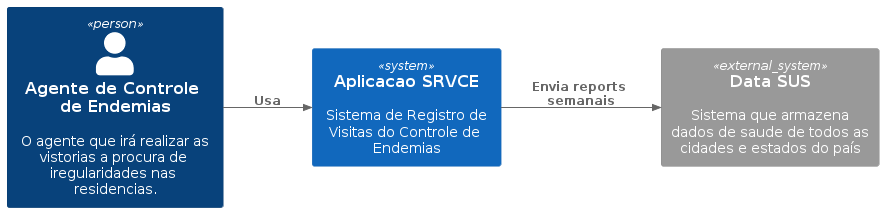
\includegraphics[height=0.5\textheight]{dados/figuras/context_map.png}
	\caption{Diagrama de Contexto. \textbf{Fonte:} Elaborado pelo Autor 2023}
\end{figure}

Em conjunto com a arquitetura Cliente/Servidor, será utilizada também a Arquitetura em Camadas. Permitindo a divisão clara das responsabilidades de cada componente dos sistemas individuais, permitindo uma melhor organização e manutenibilidade dos sistemas.

\section{TECNOLOGIAS}
Durante a escolha das tecnologias, diversos pontos foram considerados. Dentre os pontos estão a familiaridade com a linguagem, aplicações a serem desenvolvidas, o desempenho das linguagens, a comunidade de desenvolvedores para suporte ao desenvolvimento e pela robustez que os ecossistemas oferecem. 
Para desenvolvimento da aplicação servidor, foi escolhida a linguagem Java utilizando Spring Boot para realizar a construção da interface de comunicação. O framework Spring e seus derivados como Spring Boot, fornecem uma base para desenvolvimento e configuração de APIs, permitindo diversas facilidades durante o processo.
Para desenvolvimento da aplicação cliente que será utilizada em dispositivos móveis Android, foi escolhida a linguagem Kotlin, atualmente a linguagem oficial para desenvolvimento no ecossistema. Apesar de ser uma linguagem relativamente nova, possui uma vasta comunidade, além de possuir grande semelhança e interoperabilidade com a linguagem com Java, sua antecessora.
Para o armazenamento dos dados coletados durante a atividade em campo será utilizado o MongoDB, dada a natureza das atividades a serem registradas, visto que cada um dos atendimentos se encaixa como um documento.

\begin{figure}[!htb]
	\centering
	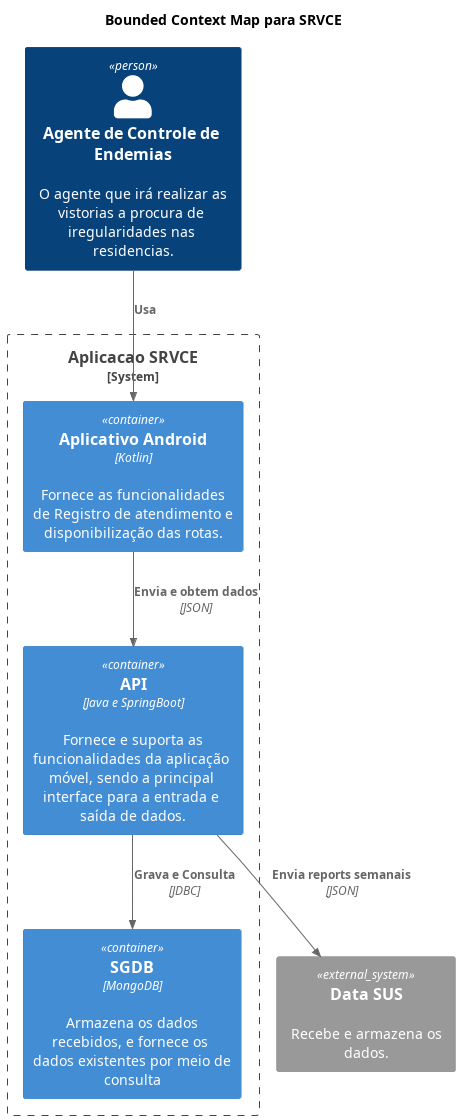
\includegraphics[height=0.5\textheight]{dados/figuras/bounded_context.png}
	\caption{Diagrama de Container \textbf{Fonte:} Elaborado pelo Autor 2023}
\end{figure}

%-----------------------------------------------------------------------------------------

%\section{REFERÊNCIAL TEÓRICO}
%\label{sec:estadoarte}

%-----------------------------------------------------------------------------------------

%\subsection{DIFERENCIAL TECNOLÓGICO}
%\label{sec:diferencial}

%-----------------------------------------------------------------------------------------

%\section{MATERIAIS E MÉTODOS} % Escolher o nome mais adequado ao trabalho
%\label{sec:metodologia}

%-----------------------------------------------------------------------------------------

%\section{RESULTADOS ESPERADOS}
%\label{sec:resultados}

%-----------------------------------------------------------------------------------------

\section{CRONOGRAMA}
\label{sec:planejamento}
% Planejamento do Trabalho----------------------------------------------------------------
% Esta seção não precisa ser editada, apenas edite o quadro 1 armazenada no diretório ".\dados\quadros"

Neste capítulo está disposto o cronograma de atividades a serem realizadas no período de desenvolvimento da proposta e aplicação da proposta. Dessa forma, cada um dos objetivos específicos citados na seção 2.3 estão alocados a um ou mais meses, dependendo da complexidade da etapa e as dificuldades envolvidas no processo. Entre eles estão as reuniões para conhecimento da rotina e das necessidades que ocorrem no processo, definição de uma arquitetura adequada, apresentação da proposta, modelagem de telas e storyboard da aplicação mobile, modelagem do banco de dados e armazenamento local e a modelagem da comunicação entre aplicações cliente e servidor.

Segue a disposição das atividades:

\begin{quadro}[!htb]
    %\centering
    \caption{Cronograma de Atividades.\label{qua:quadro1}}
    \begin{tabular}{|p{4.5cm}|p{0.7cm}|p{0.7cm}|p{0.7cm}|p{0.7cm}|p{0.7cm}|p{0.7cm}|p{0.7cm}|p{0.7cm}|p{0.7cm}|p{0.7cm}|}
        \hline
        \textbf{Atividades} & \textbf{Set} & \textbf{Out} & \textbf{Nov} & \textbf{Dez} & \textbf{Fev} & \textbf{Mar} & \textbf{Abr} & \textbf{Mai} & \textbf{Jun} & \textbf{Jul}\\
        \hline
        \small{1. Conhecimento da rotina de trabalho} & X &   &   &   &   &   &   &   &   &  \\
        \hline
        \small{2. Conhecer necessidades do processo.} & X &   &   &   &   &   &   &   &   &  \\
        \hline
	\small{3. Definir arquitetura e realizar modelagem da aplicação com escolha das tecnologias.} &   &   & X & X &   &   &   &   &   &  \\
        \hline
	\small{4. Defesa do projeto de TCC} &   &   &   &   & X &   &   &   &   &  \\
        \hline
	\small{5. Modelar as telas e o storyboard da aplicação mobile} &   &   &   &   &   & X & X  & X &   &  \\
        \hline
	\small{6. Modelar a base de dados e o armazenamento local} &   &   &   &   &   &   &   & X & X &  \\
        \hline
	\small{7. Modelar a comunicação entre a aplicação cliente e o servidor.} &   &   &   &   &   &   &   &   & X &  \\
        \hline
    	\small{8. Desenvolver versão Android.} &   &   &   &   &   &   &   &   & X &  \\
    \hline
    	\small{9. Desenvolver API.} &   &   &   &   &   &   &   &   & X &  \\
    \hline
    	\small{10. Redigir o TCC} &   &   &   &   &   &   &   &   & X &  \\
    \hline
    	\small{11. Apresentação de TCC} &   &   &   &   &   &   &   &   & X &  \\
    \hline
    \end{tabular}
\end{quadro}

%-----------------------------------------------------------------------------------------

%\section{CONCLUSÃO/CONSIDERAÇÕES FINAIS} % Escolher o nome mais adequado ao trabalho
%\label{sec:conclusao} 

%-----------------------------------------------------------------------------------------                         % Descrição da Proposta

\postextual
% INSERE ELEMENTOS PÓS-TEXTUAIS
% REFERÊNCIAS------------------------------------------------------------------

% Carrega o arquivo "base-referencias.bib" e extrai automaticamente as referências citadas

\bibliography{./base-referencias}{}
\bibliographystyle{abntex2-alf} % Define o estilo ABNT para formatar a lista de referências

% OBSERVAÇÕES------------------------------------------------------------------
% Este arquivo não precisa ser alterado.
        % Referências

\end{document}
